\documentclass[conference]{IEEEtran}
\IEEEoverridecommandlockouts
% The preceding line is only needed to identify funding in the first footnote. If that is unneeded, please comment it out.
\usepackage{cite}
\usepackage{amsmath,amssymb,amsfonts}
\usepackage{algorithmic}
\usepackage{graphicx}
\usepackage{textcomp}
\usepackage{xcolor}

\def\BibTeX{{\rm B\kern-.05em{\sc i\kern-.025em b}\kern-.08em
    T\kern-.1667em\lower.7ex\hbox{E}\kern-.125emX}}
% ============================================================
\usepackage{xspace}
\usepackage{graphicx}
% \usepackage[normalem]{ulem} % \emph should italicize, not underline
% \graphicspath{{./figures/}}
% \usepackage[pdftex,colorlinks=true,pdfstartview=FitV,
% 	linkcolor=blue,citecolor=blue,urlcolor=blue]{hyperref}
\usepackage[pdftex,colorlinks=true,pdfstartview=FitV,
 	linkcolor=black,citecolor=black,urlcolor=black]{hyperref}
\usepackage{needspace}
\newcommand{\needlines}[1]{\Needspace{#1\baselineskip}}
\usepackage{paralist}
% ============================================================
%:Markup macros for proof-reading
\usepackage{ifthen}
\usepackage[normalem]{ulem} % for \sout
\usepackage{xcolor}
\newcommand{\ra}{$\rightarrow$}
\newboolean{showedits}
\setboolean{showedits}{true} % toggle to show or hide edits
%\setboolean{showedits}{false} % toggle to show or hide edits
\ifthenelse{\boolean{showedits}}
{
	\newcommand{\meh}[1]{\textcolor{red}{\uwave{#1}}} % please rephrase
	\newcommand{\ins}[1]{\textcolor{blue}{\uline{#1}}} % please insert
	\newcommand{\del}[1]{\textcolor{red}{\sout{#1}}} % please delete
	\newcommand{\chg}[2]{\textcolor{red}{\sout{#1}}{\ra}\textcolor{blue}{\uline{#2}}} % please change
	\newcommand{\nbe}[3]{
		{\colorbox{#3}{\bfseries\sffamily\scriptsize\textcolor{white}{#1}}}
		{\textcolor{#3}{\sf\small$\blacktriangleright$\textit{#2}$\blacktriangleleft$}}}
}{
	\newcommand{\meh}[1]{#1} % please rephrase
	\newcommand{\ins}[1]{#1} % please insert
	\newcommand{\del}[1]{} % please delete
	\newcommand{\chg}[2]{#2}
	\newcommand{\nbe}[3]{}
}
%
\newcommand\rA[1]{\nbe{Reviewer A}{#1}{cyan}}
\newcommand\rB[1]{\nbe{Reviewer B}{#1}{olive}}
\newcommand\rC[1]{\nbe{Reviewer C}{#1}{magenta}}
\newcommand\ANS[1]{\nbe{Response}{#1}{teal}}
% ============================================================
%:Box comments/edits
\usepackage[most]{tcolorbox}
\ifthenelse{\boolean{showedits}}
{
  \newtcolorbox{inserted}{%
       title=Inserted text:,
       colframe=blue,colback=blue!5!white,
       breakable,
       leftrule=0mm, 
       bottomrule=0mm,
       rightrule=0mm,
       toprule=0mm,
       arc=0mm, outer arc=0mm,
       oversize
  }
  \newtcolorbox{deleted}{%
       title=Deleted text:,
       colframe=red,colback=red!5!white,
       breakable,
       leftrule=0mm, 
       bottomrule=0mm,
       rightrule=0mm,
       toprule=0mm,
       arc=0mm, outer arc=0mm,
       oversize
  }
  \newtcolorbox{refactored}{%
       % title=Heavily modifed/refactored text:,
       title=Rewritten text:,
       colframe=blue,colback=red!5!white,
       breakable,
       leftrule=0mm, 
       bottomrule=0mm,
       rightrule=0mm,
       toprule=0mm,
       arc=0mm, outer arc=0mm,
       oversize
  }
}{
  \newenvironment{inserted}{}{}
  %\newenvironment{deleted}{ \begin{comment} }{ \end{comment} }
  \let\deleted\comment
  \newenvironment{refactored}{}{} 
}
% ============================================================
%:Put edit comments in a really ugly standout display
%\usepackage{ifthen}
\usepackage{amssymb}
\newboolean{showcomments}
\setboolean{showcomments}{true}
%\setboolean{showcomments}{false}
\newcommand{\id}[1]{$-$Id: scgPaper.tex 32478 2010-04-29 09:11:32Z oscar $-$}
\newcommand{\yellowbox}[1]{\fcolorbox{gray}{yellow}{\bfseries\sffamily\scriptsize#1}}
\newcommand{\triangles}[1]{{\sf\small$\blacktriangleright$\textit{#1}$\blacktriangleleft$}}
\ifthenelse{\boolean{showcomments}}
%{\newcommand{\nb}[2]{{\yellowbox{#1}\triangles{#2}}}
{\newcommand{\nbc}[3]{
 {\colorbox{#3}{\bfseries\sffamily\scriptsize\textcolor{white}{#1}}}
 {\textcolor{#3}{\sf\small$\blacktriangleright$\textit{#2}$\blacktriangleleft$}}}
 \newcommand{\version}{\emph{\scriptsize\id}}}
{\newcommand{\nbc}[3]{}
 \newcommand{\version}{}}
\newcommand{\nb}[2]{\nbc{#1}{#2}{orange}}
\newcommand{\here}{\yellowbox{$\Rightarrow$ CONTINUE HERE $\Leftarrow$}}
\newcommand\rev[2]{\nb{TODO (rev #1)}{#2}} % reviewer comments
\newcommand\fix[1]{\nb{FIX}{#1}}
\newcommand\todo[1]{\nb{TO DO}{#1}}
\newcommand\on[1]{\nbc{ON}{#1}{red}} % add more author macros here
\newcommand\tg[1]{\nbc{TG}{#1}{orange}} % add more author macros here
\newcommand\pr[1]{\nbc{PR}{#1}{olive}} % add more author macros here
% ============================================================
\newcommand{\seclabel}[1]{\label{sec:#1}}
%\newcommand{\secref}[1]{Section~\ref{sec:#1}} <- use \autoref instead!
\newcommand{\figlabel}[1]{\label{fig:#1}}
%\newcommand{\figref}[1]{Figure~\ref{fig:#1}}
\newcommand{\tablabel}[1]{\label{tab:#1}}
%\newcommand{\tabref}[1]{Table~\ref{tab:#1}}
% ============================================================
\newcommand{\bs}{\symbol{'134}} % backslash
\newcommand{\us}{\symbol{'137}} % underscore
\newcommand{\ie}{\emph{i.e.}\xspace}
\newcommand{\eg}{\emph{e.g.}\xspace}
\newcommand{\etal}{\emph{et al.}\xspace}
% ============================================================

\begin{document}

\title{Making Systems Explainable\textsuperscript{*}\\
\thanks{* Invited keynote presentation at VISSOFT 2022.}}

\author{\IEEEauthorblockN{1\textsuperscript{st} Oscar Nierstrasz}
    \IEEEauthorblockA{
    \textit{feenk GmbH}, Wabern, Switzerland \\
    ORCID: \href{https://orcid.org/0000-0002-9975-9791}{0000-0002-9975-9791}}
\and
\IEEEauthorblockN{2\textsuperscript{nd} Tudor G\^irba}
    \IEEEauthorblockA{
    \textit{feenk GmbH}, Wabern, Switzerland \\
    ORCID: \href{https://orcid.org/0000-0002-2987-9624}{0000-0002-2987-9624}}
}

\maketitle

\begin{abstract}
What makes software systems explainable?

As we develop and maintain software, we have questions to ask about the code, but piecing together the answers remains hard.
% \meh{no good tools to answer them}. 
% \tg{I would focus on system, not code. for example, ``we have questions about the system but piecing together the answer still remains hard.''}
The main interface the classical IDE offers is a text editor for the source code.
Code, documentation, and the running system are disconnected.

In this keynote presentation, we will show how software systems can be made explainable with the help of three interacting technologies:
\begin{inparaenum}[(i)]
\item \emph{live notebooks} that can be used to create narratives that link documentation, source code, and running applications,
\item \emph{example methods} that not only perform tests, but produce live examples that can be used within narratives, to explain use cases, scenarios and features, and
\item a \emph{moldable inspector} that can be easily extended with live \emph{custom views} to answer domain-specific questions about software systems.
\end{inparaenum}

With the help of running examples we will show in the keynotes presentation how these technologies work together to provide a radically different kind of development experience.
\end{abstract}

\begin{IEEEkeywords}
Smalltalk; program comprehension; notebooks; testing; debugging
\end{IEEEkeywords}

% ============================================================
\section*{What does it mean for a system to be explainable?}

For a software system to be \emph{explainable}, it should empower developers to answer questions about it.
Questions like:
\begin{itemize}[--]
\item \emph{How does this work?}
\item \emph{Where is this feature implemented?}
\item \emph{Where is this event handled?}
\item \emph{What does this code do?}
\item \emph{How do I use this API?}
\item \emph{Where should I hook in this new feature?}
\end{itemize}

%\pr{Add other stakeholder questions}

Questions like these are not just about the code, but also about the running system, and narratives about how it works.
Furthermore, the answers often entail multiple levels of abstraction to be addressed simultaneously.
%\tg{I would add somewhere here that the answers often require access to different levels of abstraction concomitantly. }
As a consequence, an explainable system must not only be \emph{queryable} and \emph{explorable}, but it must be able to \emph{offer narratives} that link stories with source code and live objects.
These narratives serve to explain the system not only to developers, but also to other stakeholders.

% ============================================================
\section*{What prevents current systems from being explainable?}

Current IDEs are mostly focused on \emph{editing of source code}.
Sure, there are debuggers, and plugins for analysis, but the main paradigm is: stare at your code, edit it, compile, run your tests, run the code, fix bugs, repeat.

Documentation is largely static, and at most provides links to other documentation, or to source code.
Tests provide a path to live objects only if they fail, and if one is brave enough to use a debugger to explore the live program state.
Debuggers offer only low-level inspector views of the state of objects.
Various plugins may exist but such specialized tools tend not to offer ways to tailor their views to the specific questions raised within the domain of a particular application.

% ============================================================
\section*{How do we make systems explainable?}

We claim that we can make systems explainable by shifting the focus in the IDE from editing source code to exploring live objects, source code, and narratives that link them.
Such an IDE would allow us to seamlessly navigate between these three aspects.

%:MD
Glamorous Toolkit,\footnote{\url{https://gtoolkit.com}} or \emph{GT}, is a \emph{moldable} development environment which is designed so that its tools can be easily ``molded'' to the needs of a particular domain or application.
Although there are many parts to GT, the key components for making systems explainable are
\begin{inparaenum}[(i)]
\item a live notebook (Lepiter) that allows developers to construct interactive narratives about code and live objects,
\item a coding environment (aka ``Coder'') that links source code to live examples, and
\item a moldable object inspector (Inspector) that allows developers to cheaply add custom views for exploring and navigating the web of objects of a domain.
\end{inparaenum}

These components make systems explainable by enabling querying, navigation and story-telling for developers, and also for other stakeholders.

% ============================================================
\section*{Really? Explain the pieces to me}

% ------------------------------------------------------------
\subsection{Lepiter}

Lepiter~\cite{Girb21a} is a live notebook, connecting documentation of models and source code with live, running examples.

\begin{figure}[htbp]
  \centering
  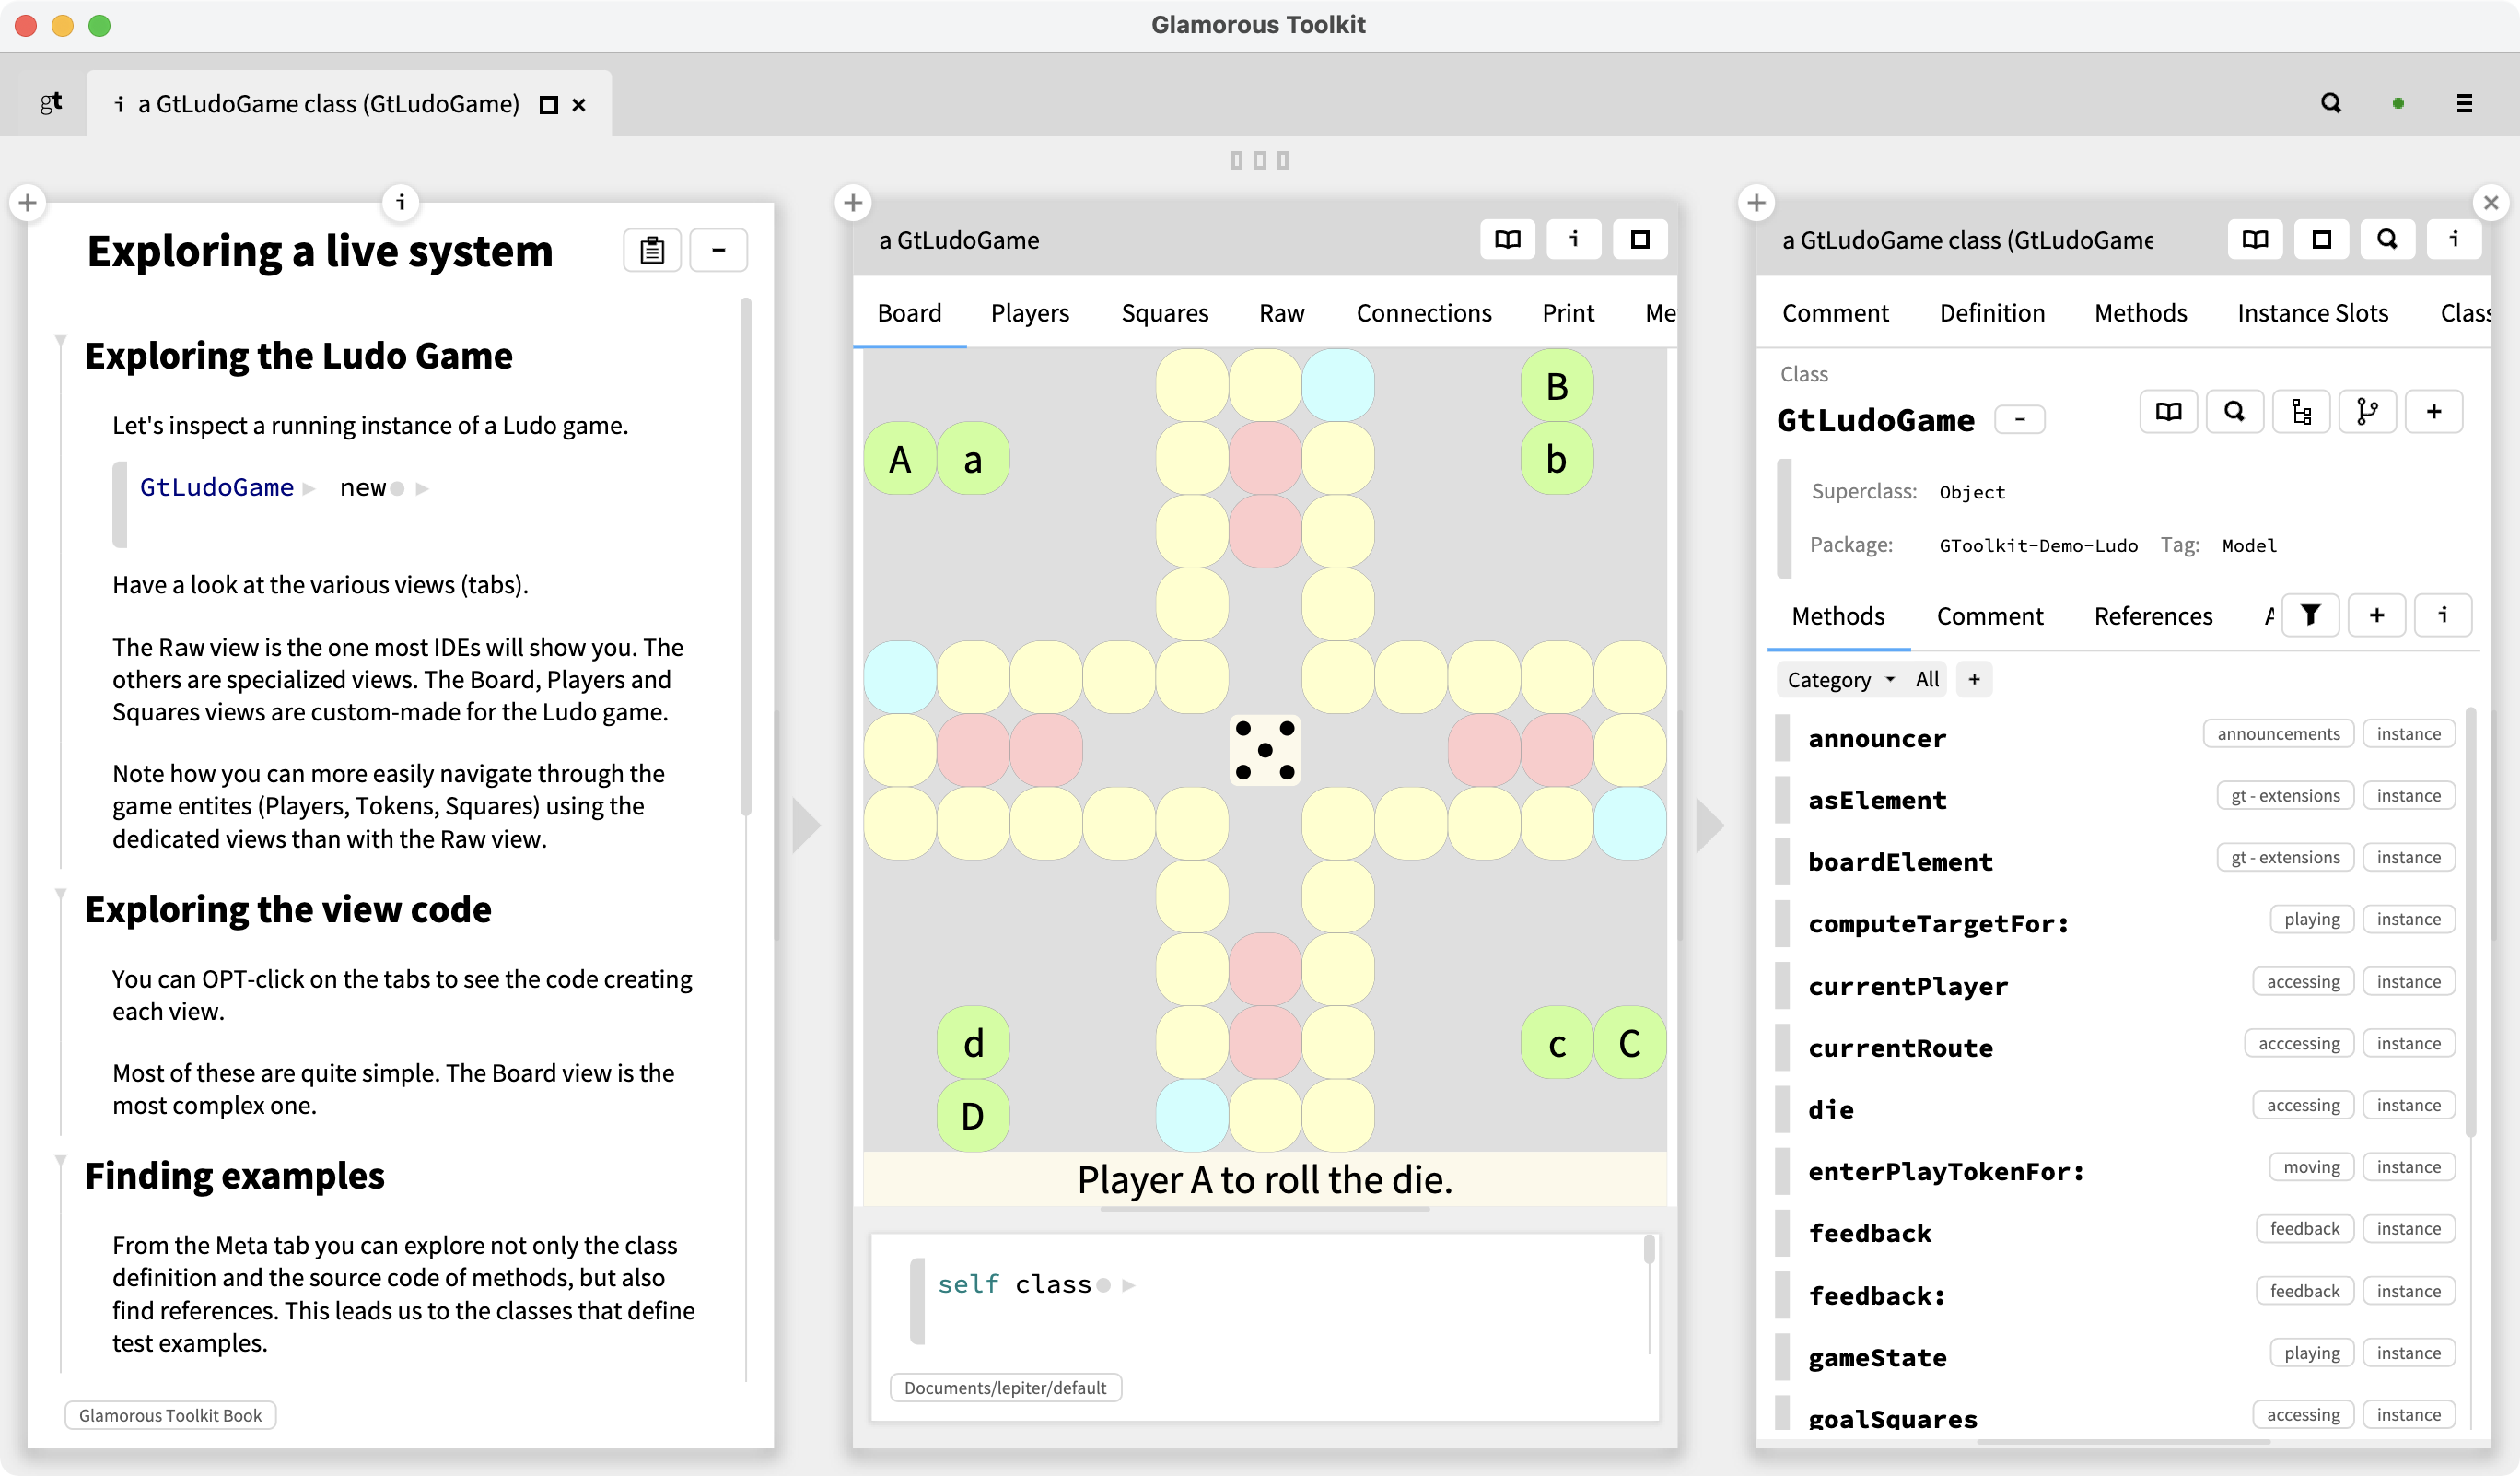
\includegraphics[width=\columnwidth]{figures/note-inspector-coder.png}
  \caption{Navigating from a Lepiter note to a custom view of live instance, and from there to the source code.}
  \figlabel{note-inspector-coder}
\end{figure}

Pages in a notebook consist of linked text interspersed with various kinds of snippets, such as embedded code, live visualizations, and code snippets that can be evaluated.
As in the Coder and the Inspector, one navigates from view to view with the help of Miller Columns,\footnote{\url{https://en.wikipedia.org/wiki/Miller_columns}} so from a given page, one can navigate to another Lepiter page, a Coder view of a class or method, or an Inspector view of a live object (\autoref{fig:note-inspector-coder}).

One can therefore create narratives either by
\begin{inparaenum}[(i)]
\item telling stories in Lepiter pages, or
\item following a trail of cascading views.
\end{inparaenum}

% ------------------------------------------------------------
\subsection{Examples}

Examples are live objects produced by executing \emph{example methods}\cite{Gael03c,Gael07a,Girb19a}. 

Example methods are just like unit tests, except that they return an object instead of simply passing or failing.
This means that the result of a test is not just a status report, but a \emph{live object} that can be explored.

An example can be used as input to another example method, thus allowing tests to be chained.
(So when a test fails, its dependent tests don't fail, as they are not run\cite{Kuhn08a}.)

Examples can be used to create narratives, to explain use cases, scenarios and features.
Since examples can be chained, it is possible to create a chained sequence of examples that illustrate a particular scenario.
Such examples can also be embedded into a notebook page that documents and explains the steps of the scenario, while linking to the live, explorable instances (\autoref{fig:composing-tests}).
%\tg{Another example could be to show the example and the representation as part of the same page, rather than two distinct panes}
%\on{sure, but for this paper I think the added value is minimal}

\begin{figure}[htbp]
  \centering
  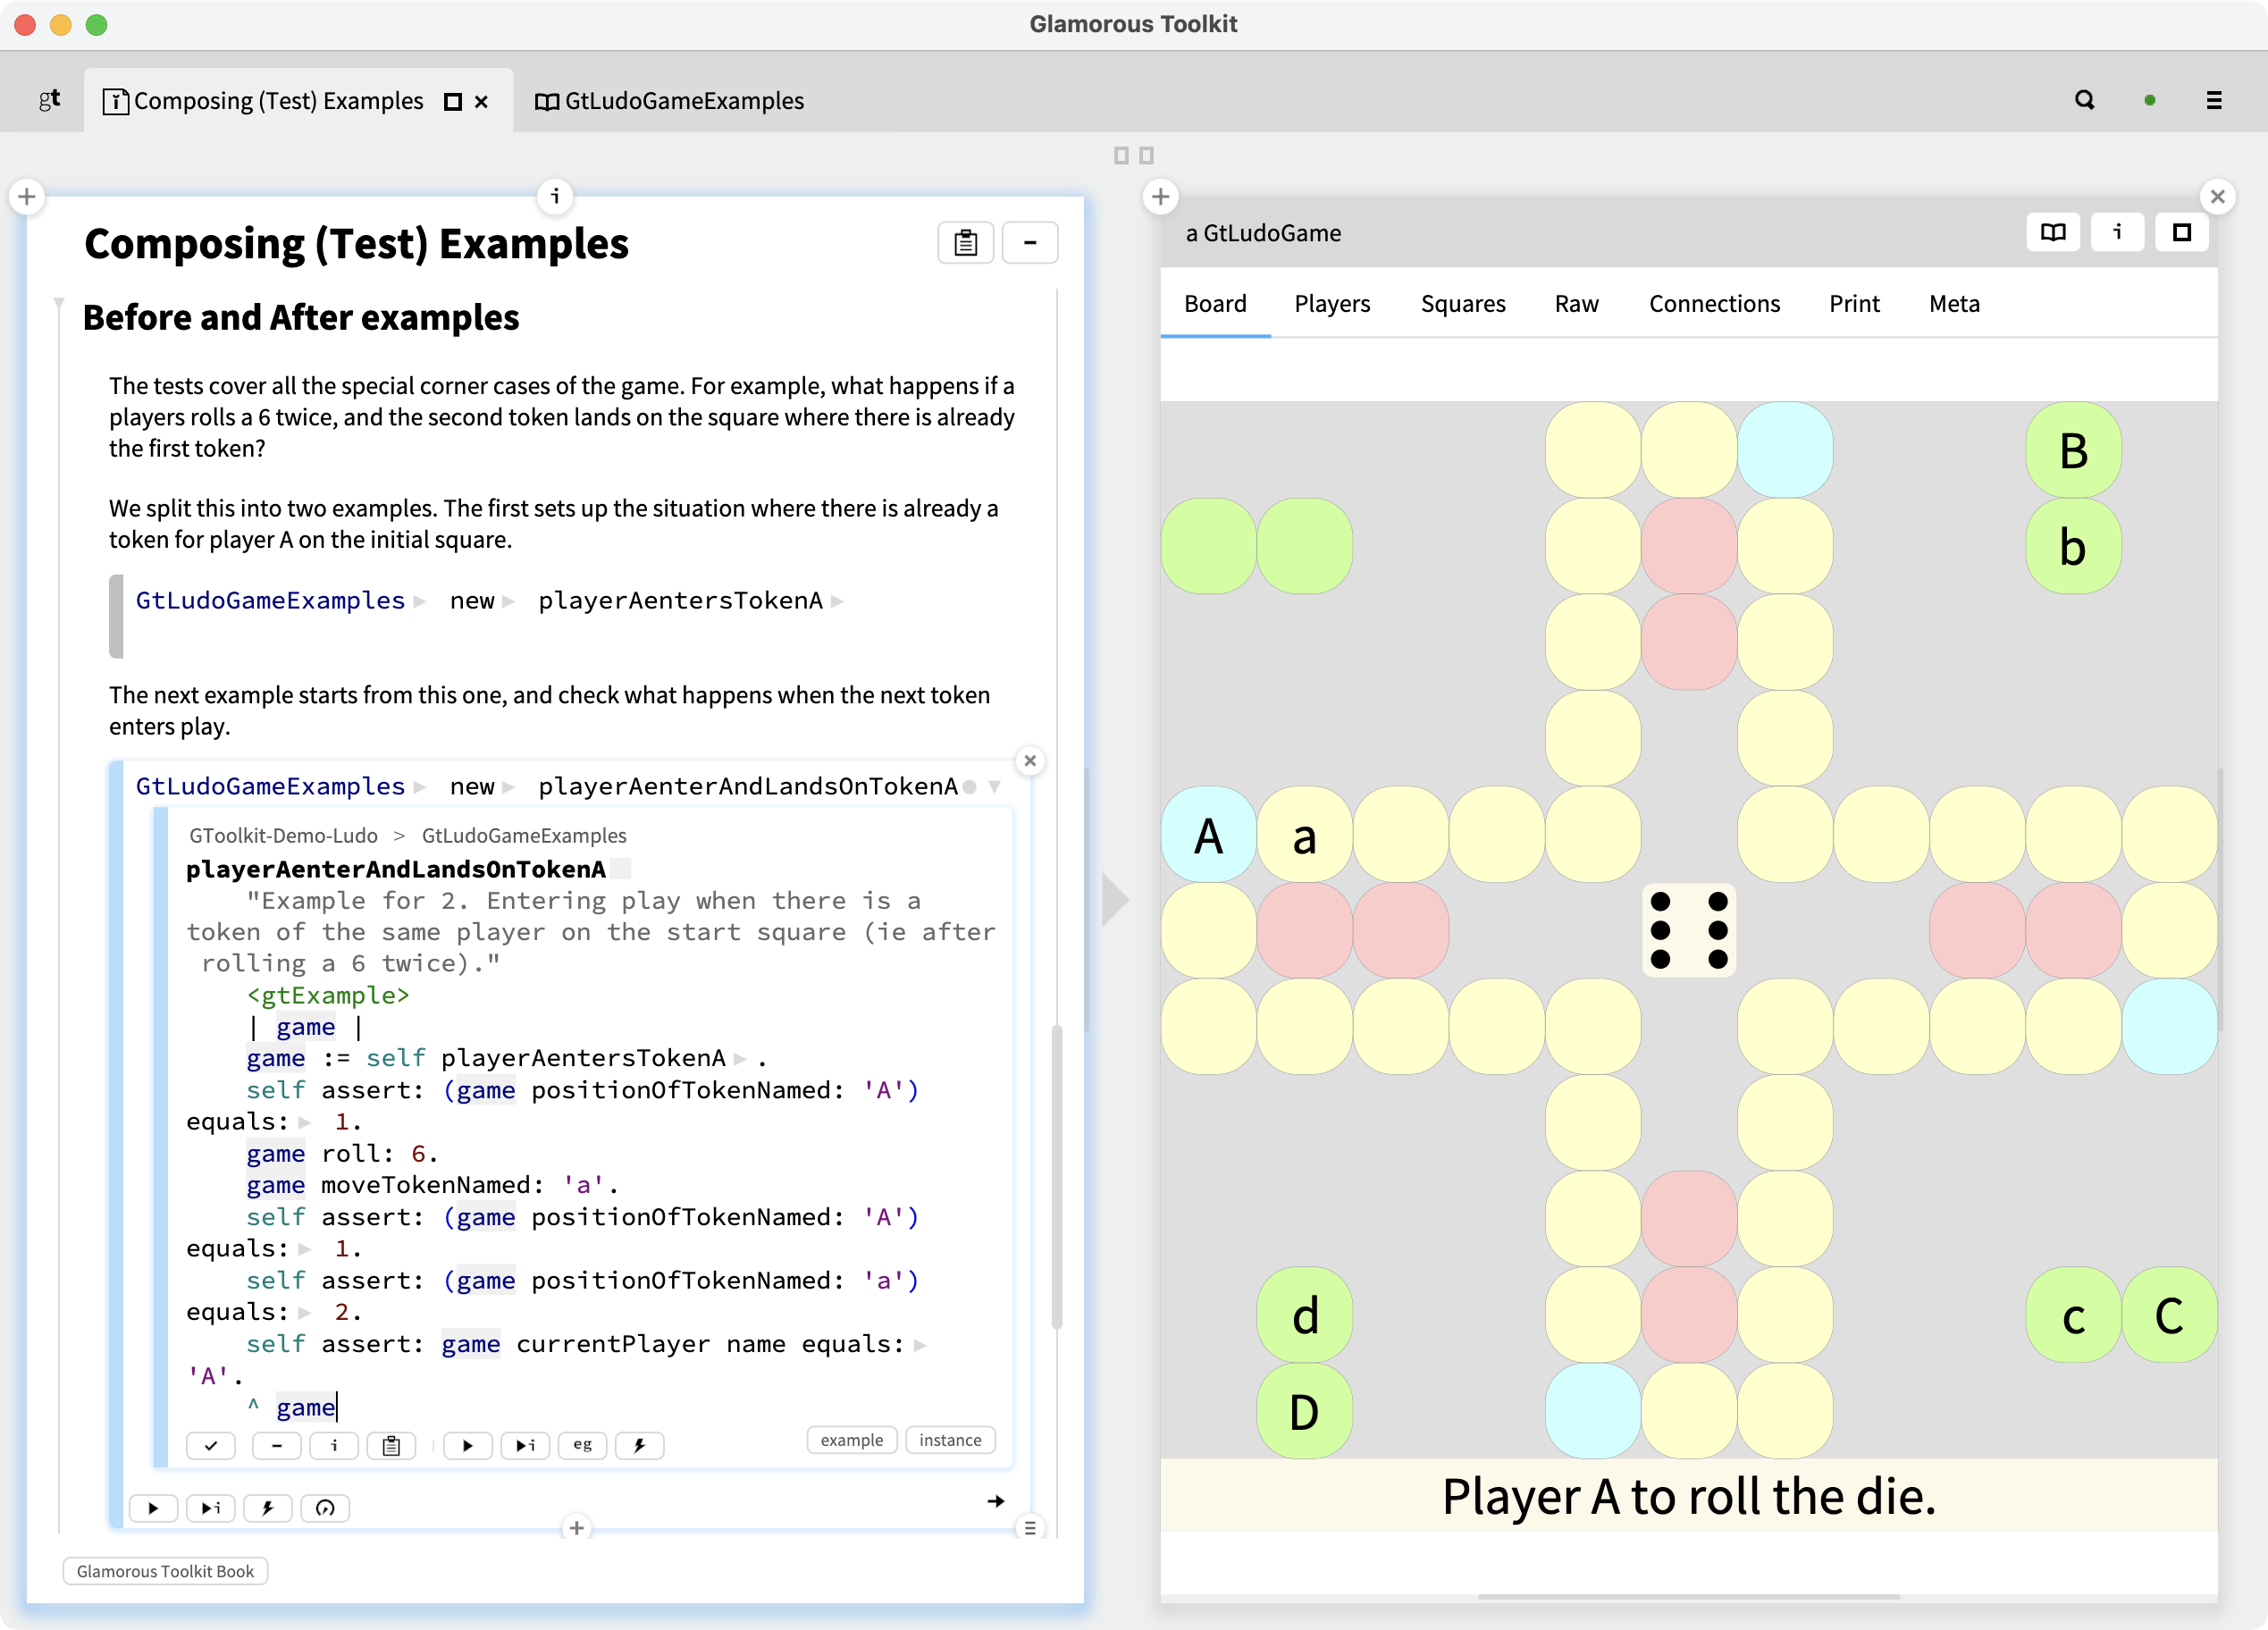
\includegraphics[width=\columnwidth]{figures/composing-tests.png}
  \caption{Explaining a scenario by composing examples that illustrate steps in a computation}
  \figlabel{composing-tests}
\end{figure}

% ------------------------------------------------------------
\subsection{The Moldable Inspector}

%\tg{This part should be rewritten a little as it is misleading:
%- the inspector is not separate from lepiter, it is part of the same environment. it is the environment that offers the miller columns.
%- the playgrounds are full lepiter pages and can host object specific narratives.}

The Inspector~\cite{Chis15a} extends the usual debugging object inspector with interactive playgrounds, Miller columns and custom views.
Rather than being an incidental tool that is only used in a debugging context, the Inspector serves as the environment in which the other tools live, as \emph{we are always inspecting some kind of object}.
The Miller columns are the primary mechanism for navigating through a chain of connected objects.
Each column provides a view of an object, and a playground that allows you to send messages to that object. 
Each playground is, in turn, a complete Lepiter page that can combine annotated text, live code snippets, and other entities.
As a consequence the Inspector offers two ways to navigate.
You can either click in the interactive view to open another view in the adjacent column, or you can evaluate a code snippet (or follow a link) to inspect the result in new column.

The Inspector is \emph{moldable} in the sense that it can be cheaply extended with \emph{custom views} that are specific to a given context (be it a domain, an application, or even an individual object) during development.~\cite{Chis17a,Chis16b}.
The key insight is that every software system raises its own questions and issues, so generic views are less likely to be helpful in making such systems explainable.
By making it easy and cheap to add custom views, the Inspector is elevated from being an obscure debugging aid, to a central tool for exploring and explaining complex software systems.

Whereas live interactions and playground queries provide a way to navigate through a web of connected objects, custom views do the opposite!
Each custom view consists of 
\begin{inparaenum}[(i)]
\item an encapsulated query, to produce the object(s) of the view, and
\item a simple, interactive visualization of the result.
\end{inparaenum}
Thus, the point of custom views is to enable developers to quickly find answers to common questions just by selecting the tab of interest, without having to navigate or code a query (\autoref{fig:custom-views}).

\begin{figure}[htbp]
  \centering
  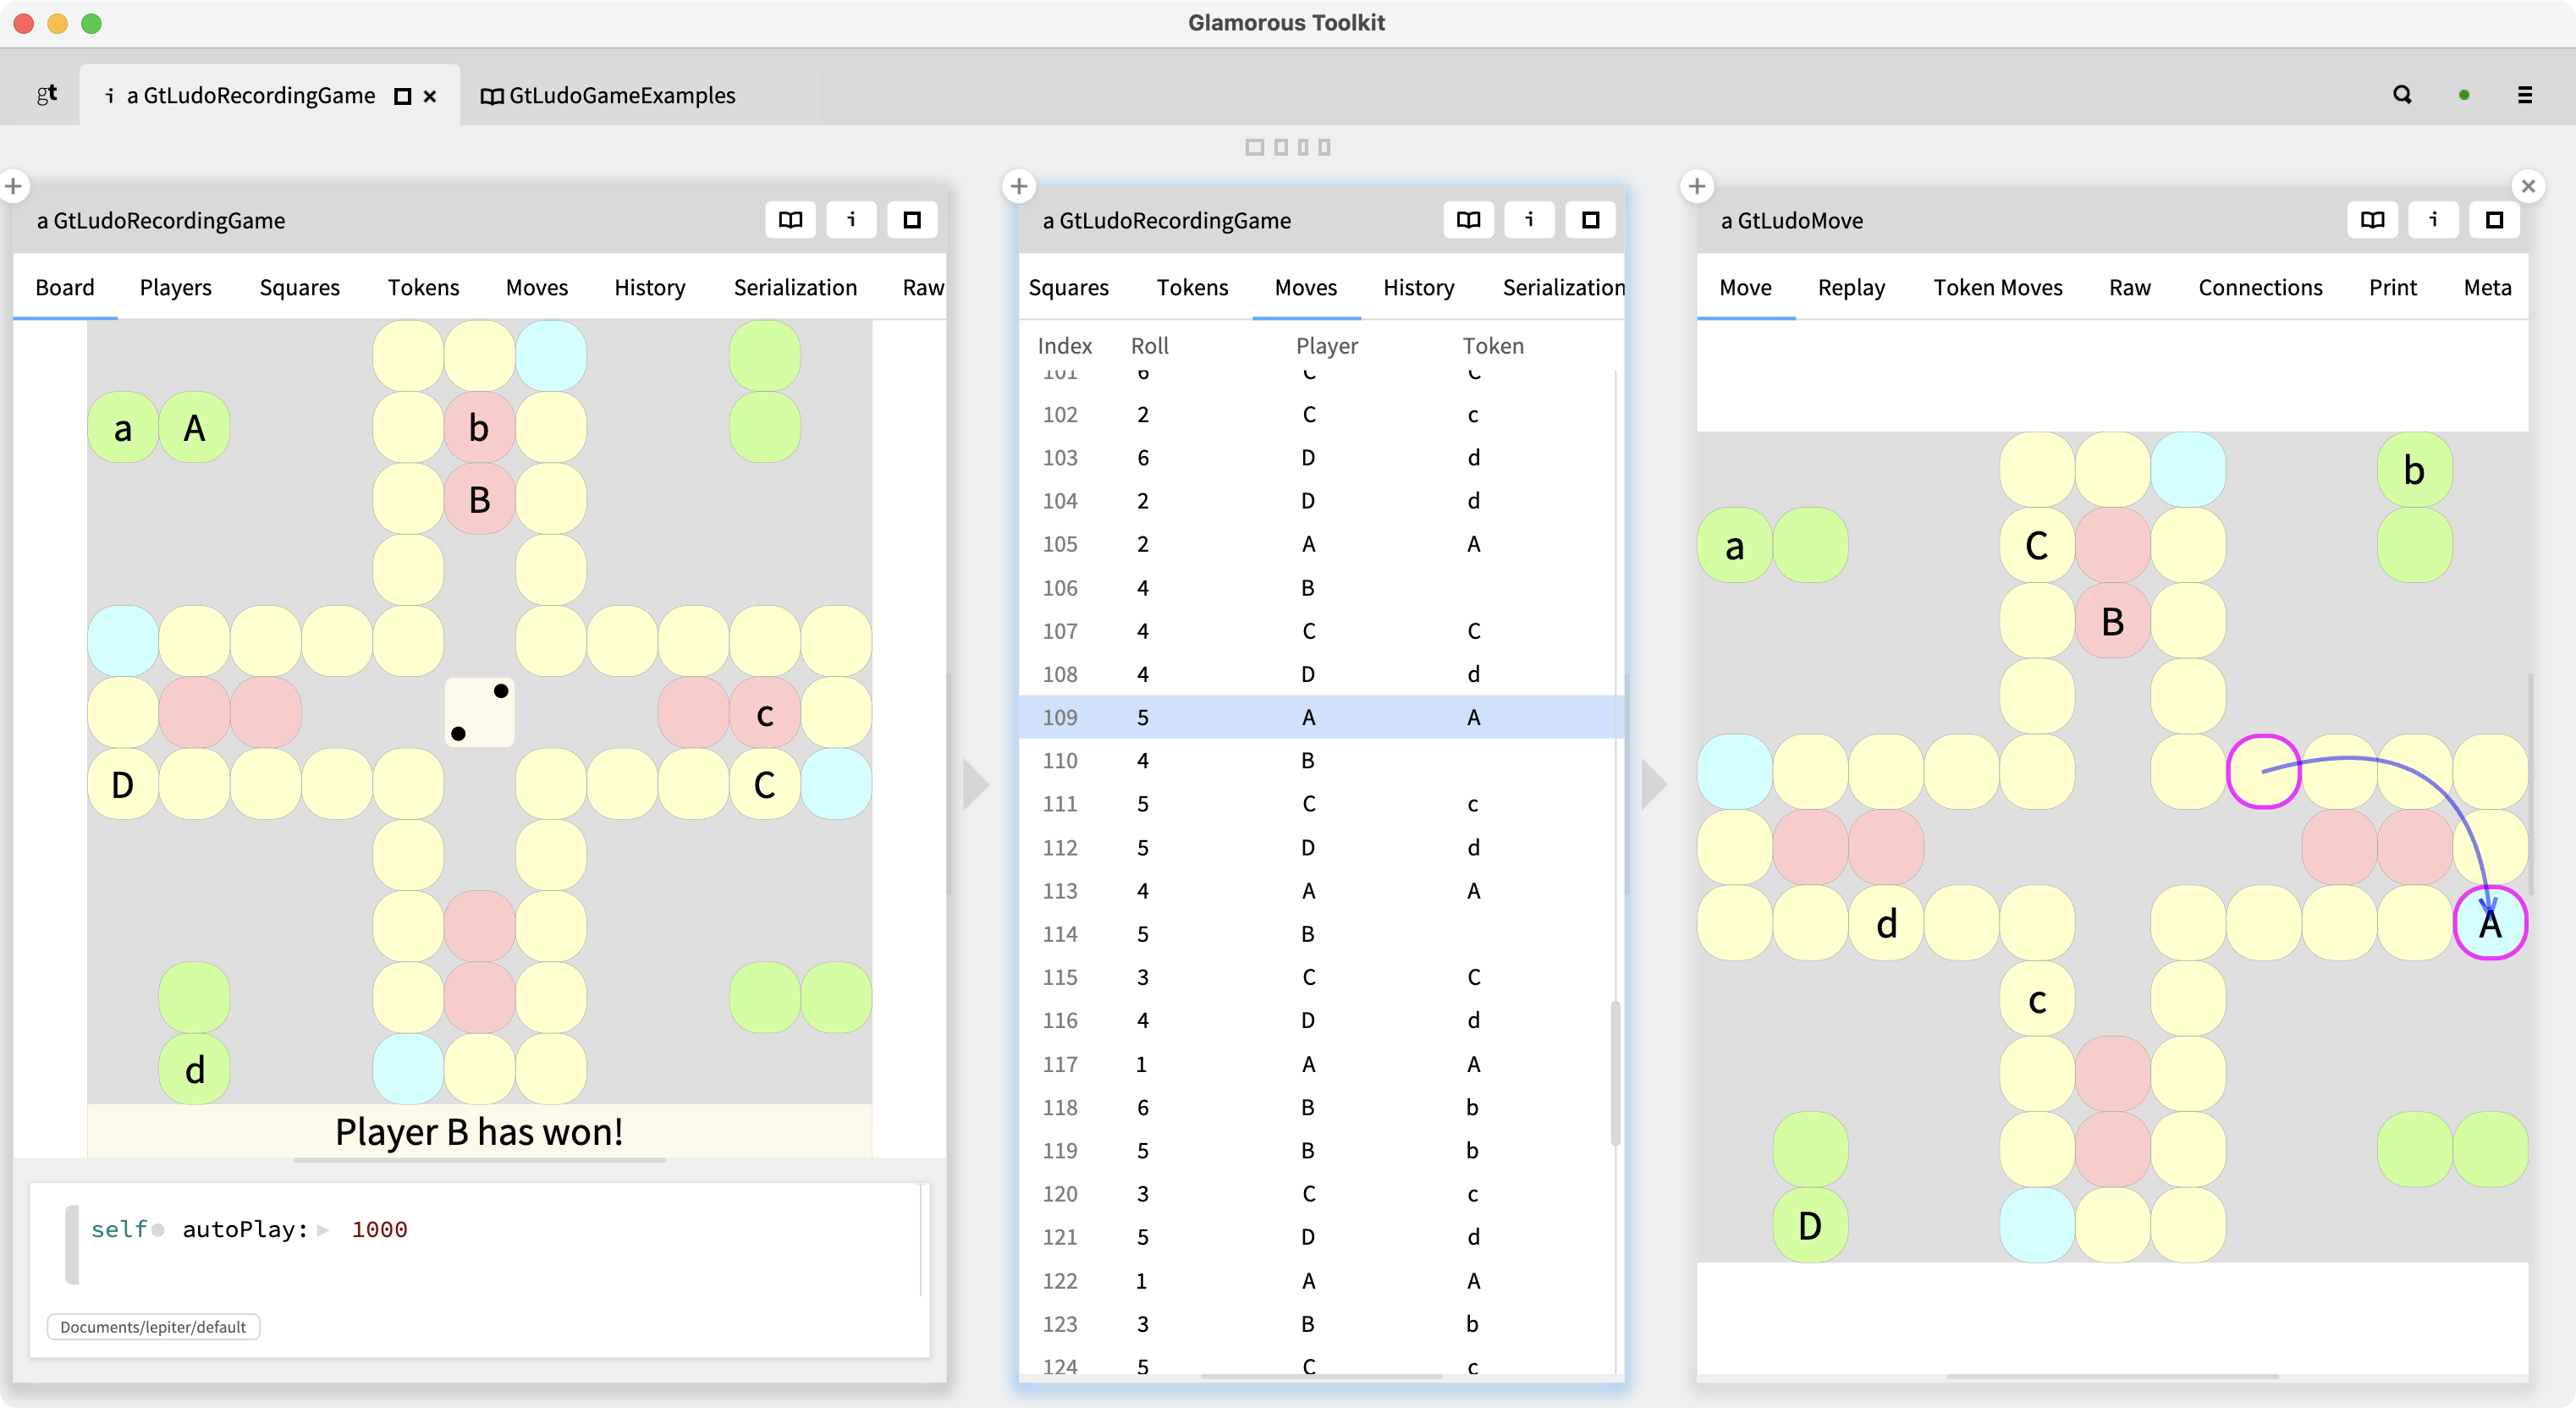
\includegraphics[width=\columnwidth]{figures/custom-views.png}
  \caption{Custom views of a Ludo game object and its moves help to explain the game logic}
  \figlabel{custom-views}
\end{figure}

% ============================================================
\section*{Why is it cheap to build custom views?}

Tools are only effectively moldable if it is cheap to adapt them.
In the current release of GT,\footnote{DEV v0.8.1735, 26 July 2022} there are 1974 custom GT views, consisting of 22\,932 lines of code, or just short of 12 lines per view.
Of course there is a lot of heavy lifting being done somewhere else, but in practice, with a bit of experience, these views are easy to create (\autoref{fig:custom-python}).

\begin{figure}[htbp]
  \centering
  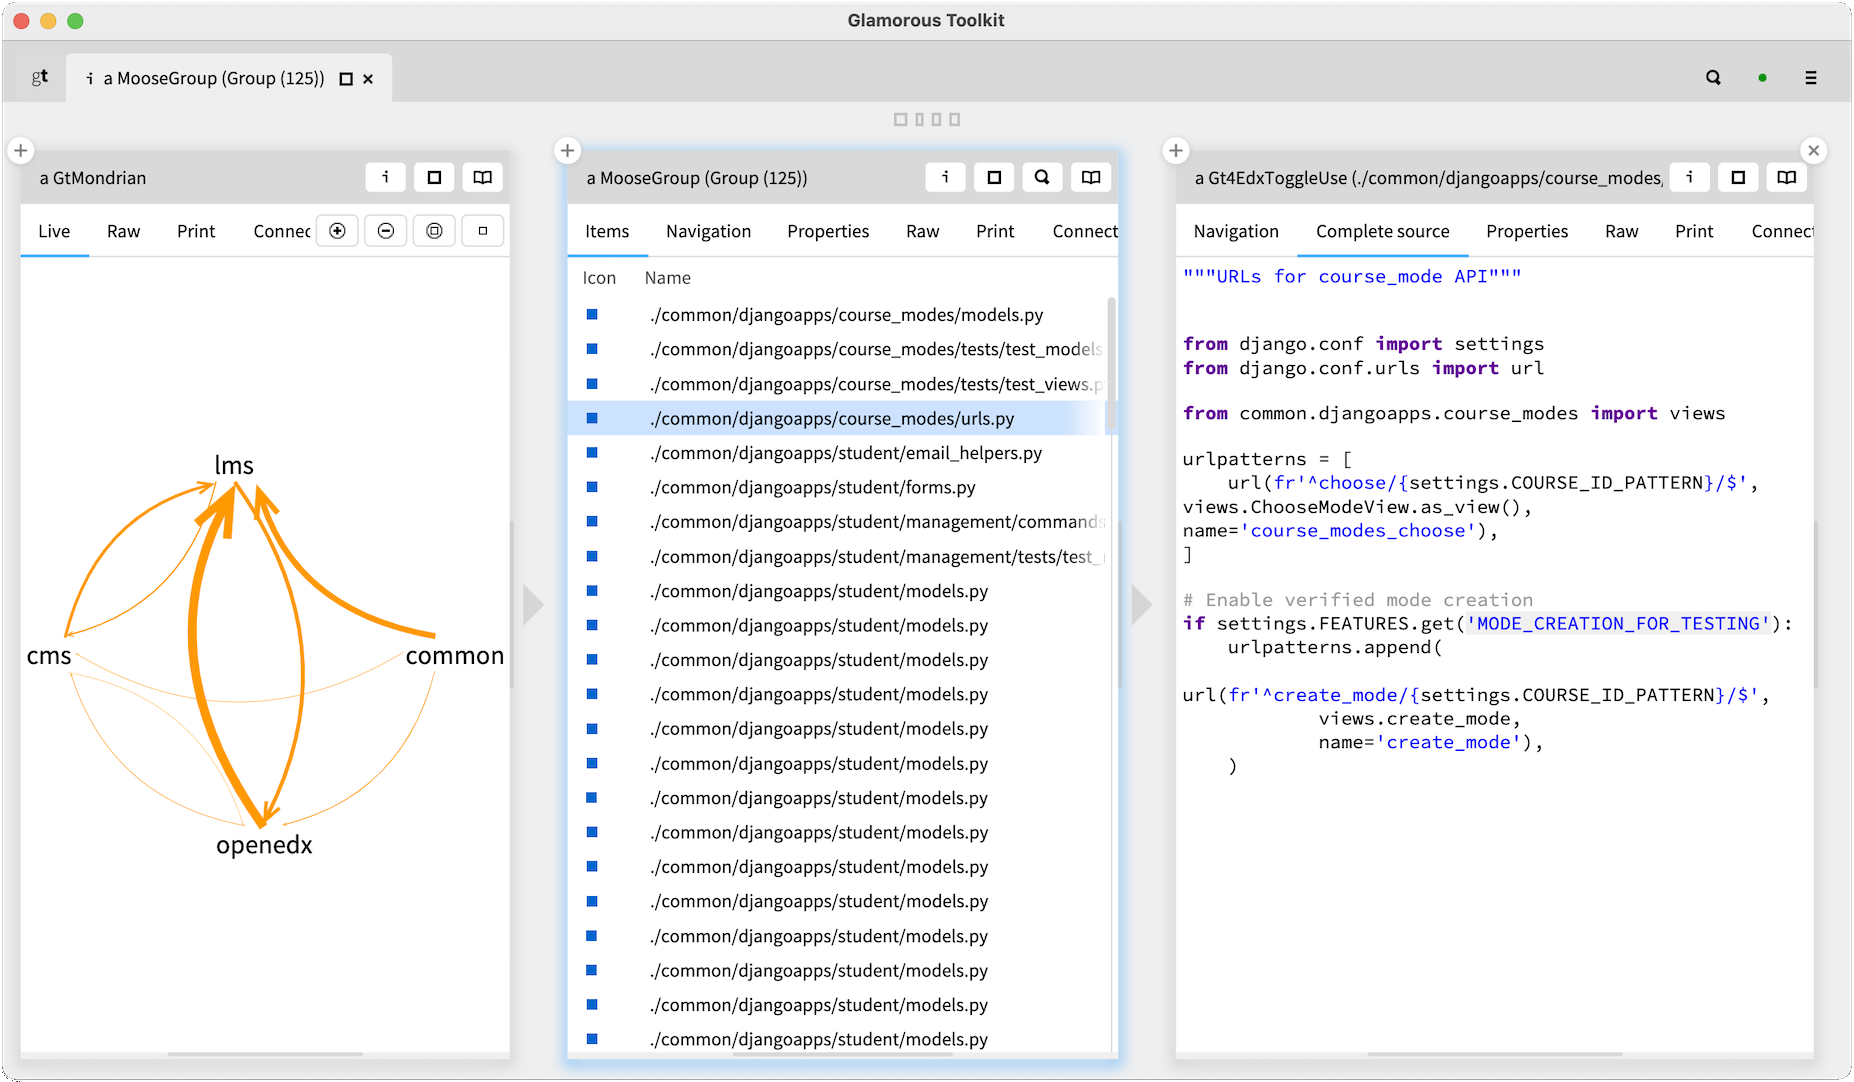
\includegraphics[width=\columnwidth]{figures/gtr-edx-dependencies-source.png}
  \caption{Custom views for static analysis of a Python project}
  \figlabel{custom-python}
\end{figure}

The key insight, however, is that GT is built with a graphical stack that has just \emph{one rendering tree}~\cite{Girb20a}.
This makes it easy to create flexible visualizations combining arbitrary elements, \ie. text, graphics, and widgets.

%\on{Here it might be nice to show a cool visualization of a non-smalltalk system}

% TG suggests https://lepiter.io/feenk/steering-agile-architecture-by-example--th-e2p6aps2brbby94deek31xqxh/attachments/bo6wwplvc3aos7iz21hqoed73/gtr-edx-dependencies-source.png
% This is described in https://lepiter.io/feenk/steering-agile-architecture-by-example--th-e2p6aps2brbby94deek31xqxh/

% ============================================================
\section*{How does all this impact software development?}

Just like testing should not be an afterthought, \emph{making systems explainable should be part of the development process}.

In short, you should:
\begin{inparaenum}[(i)]
\item document narratives about the software you are building as well the process you are following itself,
\item create meaningful examples as you develop, and
\item create customs views to expose what's important.
%\tg{I would be more explicit about moldable development: the key is the inversion of flow: whenever we have a question, we devise a custom narrative to make the problem explicit. It’s the narrative that drives the rest.}
\end{inparaenum}


\begin{figure}[htbp]
  \centering
  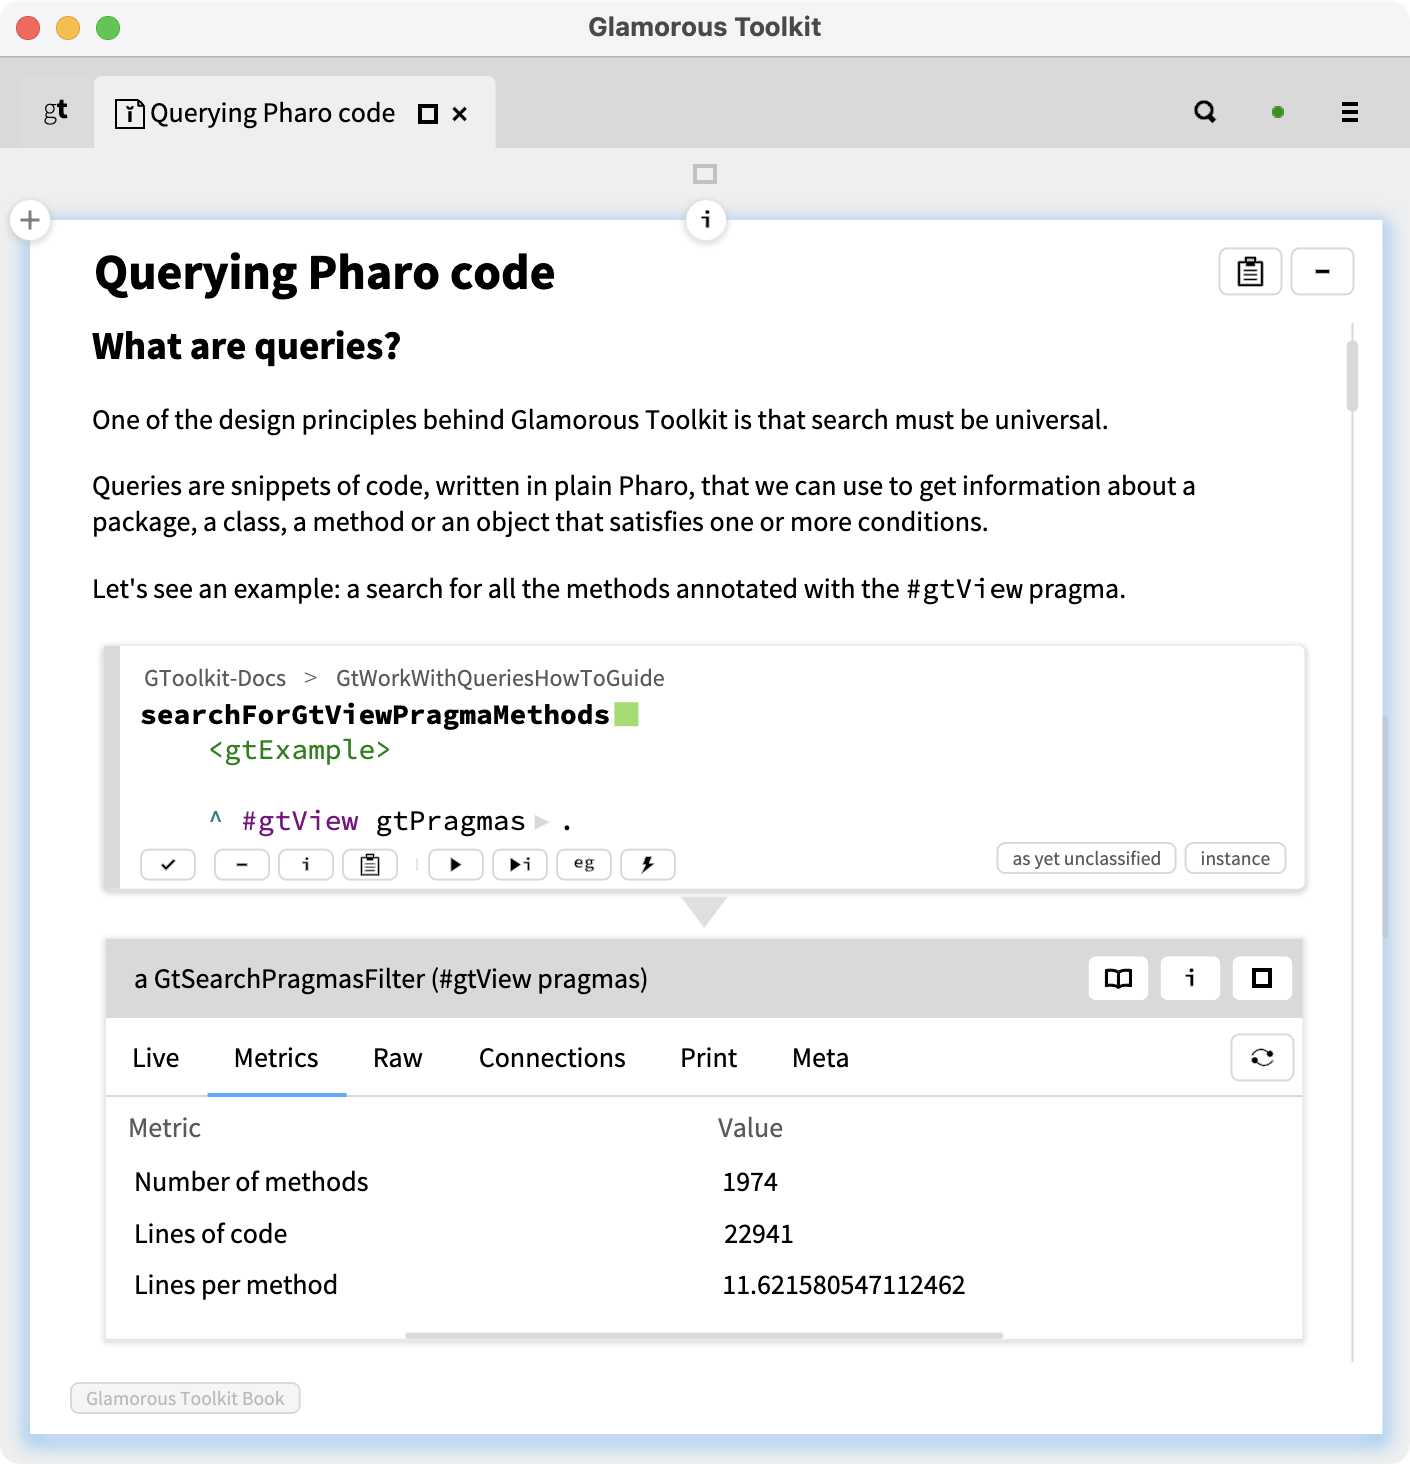
\includegraphics[width=\columnwidth]{figures/querying-pharo-code.png}
  \caption{Querying Pharo code}
  \figlabel{querying-pharo-code}
\end{figure}


\emph{Lepiter} influences development in several ways:
Live documentation is not an add-on, but an integral part of a software system.
Lepiter is the single starting point for most development tasks. 
For example, we used a Lepiter page even to find out how many custom views there are in GT (\autoref{fig:querying-pharo-code}).
Systems become explainable by linking code and examples in live documentation.
Creating narratives that consist of live documentation becomes part of the development process.
As you develop software, you document your process by creating tagged notes that describe features and use cases, while linking code and examples.
Whenever we have a question, we devise a custom narrative to make the problem explicit. 
It’s the narrative that drives the rest. 
%:MD
This is the essence of what we call Moldable Development.\footnote{\url{https://moldabledevelopment.com}}


\emph{Examples} also form a key component of both the software and the process:
Example-driven development\cite{Girb19a} forces you to develop the system in a way that it can be explored, visualized and explained, just like TDD encourages you to develop systems so they become testable!
If you need a feature, write an example (test).
If you find a bug, write an example.
If you want to explain something, write an example.

Finally, \emph{custom views} reach their potential if they are introduced as the need for them arises:
If you need to navigate or write a query, create a view.
If you need to explain something about a domain concept, create a custom view.
Apply the principles of GQM (Goal - Question - Metric) to developing custom views --- don't introduce a view just because an easy visualization is available, but because there is a demonstrated need arising from domain-specific questions.
These questions may come from the developers, but they may also come from the customer, the user, or other stakeholders.
Create the views as you develop to enhance both debugging and documentation.
Custom views answer questions about domain objects in an application. 
These answers become words in narratives in live notebooks, to make systems explainable.

% ============================================================
\section*{Is that all there is?}

Well, no.
There are many other important components that help to make systems explainable with GT.
For example, \emph{Spotter}\cite{Chis16a} is context-aware tool that helps you search for anything in the IDE.
GT is also a language workbench powered by the mature \emph{SmaCC} compiler-compiler framework that enables the reverse engineering, parsing and editing of foreign languages~\cite{Bran17a}.
All these are integrated in a uniform environment made out of visual and interactive operators that can be combined to create many unexpected development experiences.

%:MD
GT is an enabling technology for Moldable Development.
Once we can explain the inside of systems, we get to unlock new opportunities at the level of the development process and even for how we create new business value.

% ============================================================
\section*{So, how would you sum that up?}

Systems become explainable by making it easy to create narratives that link documentation, code, and live objects.
This means that domain concepts become explicit, so it is easy to navigate between concepts and their instances, and it is easy to have dedicated views that expose the underlying concepts.

Instead of seeing a software system as a static collection of source code files, it should be responsive and live, integrating narratives about the code and the running application.
Alternatively, if the application is the analysis of a foreign codebase, the resulting analysis model should be equally live and responsive.

The result is that an explainable system is one which supports a \emph{dialogue} between the developer and the system.
The narratives and the views arise from the questions developers ask of the system.

% ============================================================

\subsection*{Acknowledgments}
We thank Pooja Rani for her feedback on a draft of this paper.

% ============================================================

\bibliographystyle{IEEEtran}

\bibliography{explainableSystems}

\end{document}
% ============================================================

